\section{Solving Linear Systems}

\subsection{Gauss's Method}

\begin{definition}[Linear combinations]
    A \textit{linear combination} of $x_1, x_2,...,x_n$ has the form
    \[a_1x_1 + a_2x_2 + ... + a_nx_n\]
    where the numbers $a_1,...,a_n \in \mathbb{R}$ are the combination's \textit{coefficients}. A \textit{linear equation} in the variables $x_1,...,x_n$ has the form $a_1x_1 + a_2x_2 + ... + a_nx_n = d$ where $d \in \mathbb{R}$ is the \textit{constant}.

    An \textit{n-tuple} $(s_1,s_2,...,s_n) \in \mathbb{R}^n $ is a \textit{solution} of, or \textit{satisfies}, that equation if substituting the numbers $s_1,...,s_n$ for the variables gives a true statement: $a_1s_1 + a_2s_2 +...+a_ns_n = d$. A \textit{system of linear equation}
    \[
        \begin{aligned}
            a_{1,1}x_1 + a_{1,2}x_2 + \cdots + a_{1,n}x_n & = d_1        \\
            a_{2,1}x_1 + a_{2,2}x_2 + \cdots + a_{2,n}x_n & = d_2        \\
            \vdots    \qquad  \qquad \qquad \qquad        & \quad \vdots \\
            a_{m,1}x_1 + a_{m,2}x_2 + \cdots + a_{m,n}x_n & = d_m        \\
        \end{aligned}
    \]
    has the \textit{solution} $(s_1,s_2,...,s_n)$ if that \textit{n-tuple} is a solution of all of the equations.
\end{definition}

Find the set of all solutions is \textit{solving} the system.

\begin{definition}[Elementary operations]
    If a linear system is changed to another one by one of these operations
    \begin{itemize}
        \item an equation is swapped with another
        \item an equation has both sides multiplied by a nonzero constant
        \item an equation is replaced by the sum of itself and a multiple of another
    \end{itemize}
    then the two systems have the same set of solutions.
    These operations are known as the \textbf{elementary operations}.
\end{definition}

\begin{definition}[Leading variable]
    In each row of a system, the first variable with a nonzero coefficient is the row's \textbf{leading variable}. A system is in \textbf{echelon form} if each leading variable is to the right of the leading variable in the row above it, except for the leading variable in the first row, and any rows with all-zero coefficients are at the bottom.
\end{definition}


\subsection{Exercises}
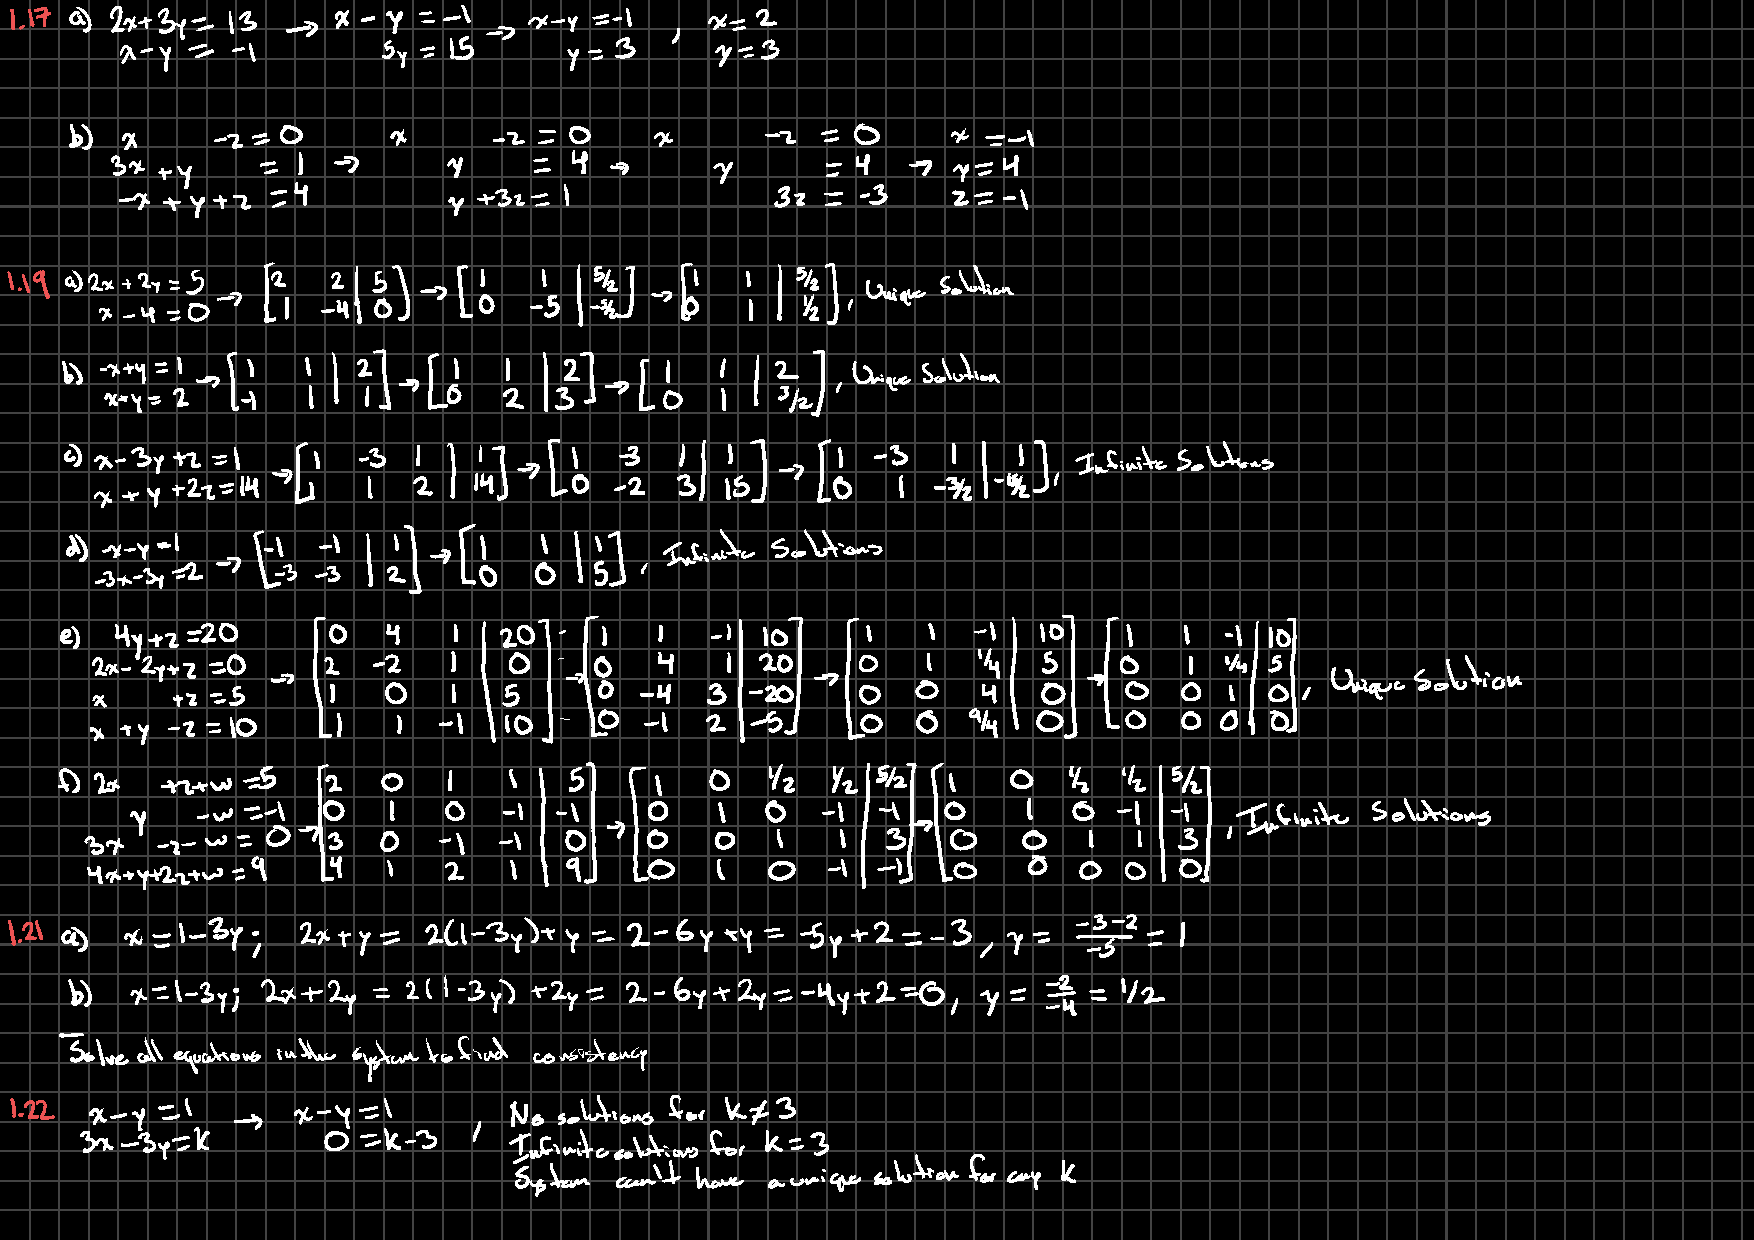
\includepdf[pages=-]{Exercises/01_Linear_Systems/01_Solving_Linear_Systems.pdf}